\chapter{Research}
With the writers lack of experience in writing applications of this type, the research phase explored a number of different avenues and began with very little in terms of preconceptions. 

\section{Similar Applications}
Initial focus was directed towards exploring existing applications that performed a similar task to gain some insight as to the expectations of the project. A number of applications that provide recognition from input devices such as the camera, microphone and other peripherals were examined.

\colorbox{red}{Three classes of application server, client/server, client only discussed below}

\subsection{Google Goggles}
With the release of the Android operating system Google have been exploring a number of user interaction mechanisms for the system. Of these alternative approaches they have had much success with the impressive \textbf{Google Voice Search}, which enables the user to command the device using their voice without any form of training.

Google have also invested resources into the development of a visual search system which they call \textbf{Goggles}. Just like Voice Search, Goggles performs very little processing on mobile handset, instead opting to transmit the data to a back-end service for processing.

Due to the commercial and proprietary nature of the product implementation details are hard to come across, but in August 2010 Google delivered a presentation at the Hot Chips conference in Stanford University that gives insight into some elements of the design of the service. During this talk Google discussed a number of interesting points, firstly due to level of processing involved and network latencies on current generation cellular networks a image search query takes in the region of about 6.5 seconds for the system to return a result to the handset. Google also broadly discussed the architecture of the back-end search processing, when an image is received by the remote server it is in parallel analysed by a number of engines. Each of these engines are tuned for extracting particular information from an image, for example they have a barcode, text, landmark, wine label and logo engine to name a few, currently it is estimated that a search is executed on 20 engines in parallel and each result is ranked with only the most confident being returned to the user \cite{vbgoggles10, sbs10}.

\begin{figure}[h!]
\centering
    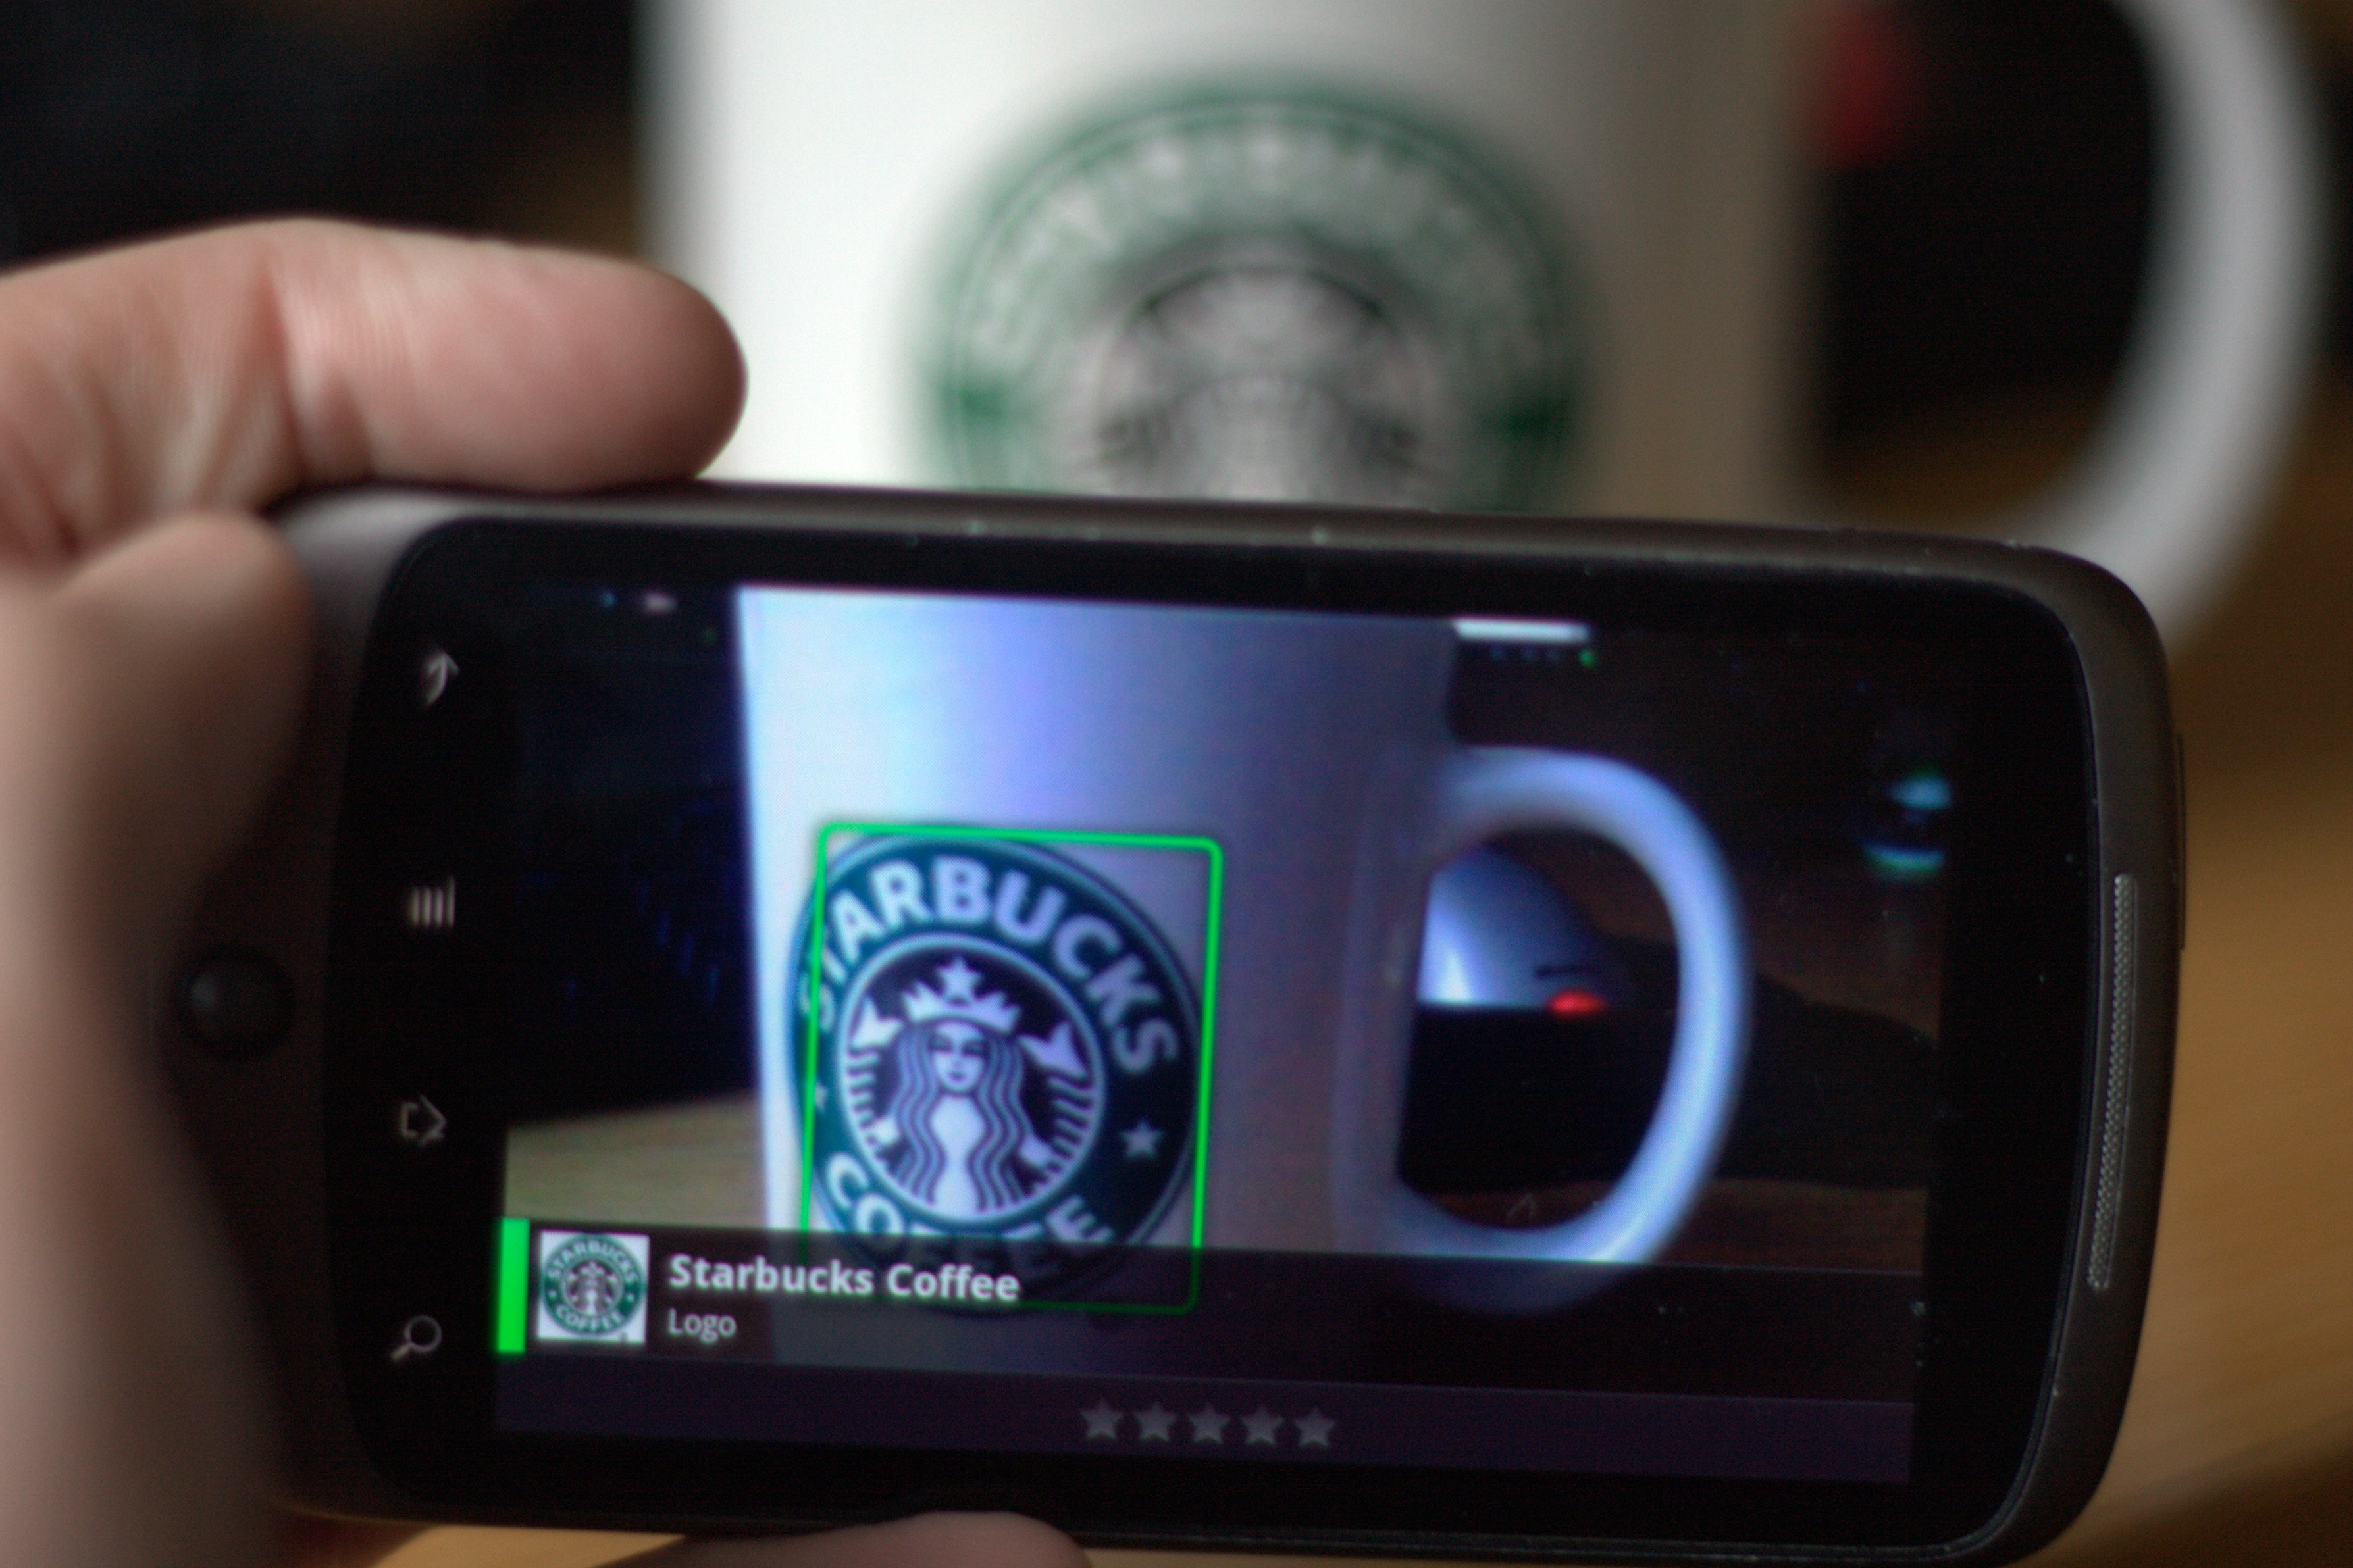
\includegraphics[width=0.7\textwidth]{research/images/goggles_example.jpg}}
	\caption[Google Goggles example]%
    {Google Goggles successfully identifies a well known logo from a coffee mug.}
\end{figure}

Google presented at the Hot Chips conference to raise awareness of the necessity to maximise the amount of processing done in the device to chip manufacturers in order to counter the latency inherent in cellular networking.

Interestingly they also discussed the use of data from other sensors to increase the context of the image, for example including geographical coordinates with an image of the Eiffel Tower could potentially aid in a more speedy result being returned.

Goggles is not currently successful at identifying instances of particular classes of objects. In their documentation they specifically mention not having a high success rate when recognising objects such as tree leaf types, animals or cars. Another major drawback is the estimated 6.5 second average response time, but this is largely bourne from transmitting the unprocessed image over the network which encompasses issues out of the control of device makers.

\subsection{Shazam}

While on initial review it may seem that Shazam is unrelated to the current project, a closer inspection reveals many similarities. Shazam is a application and back-end service which allows its users to identify a piece of music based on a short sample potentially recorded in a noisy environment with a sub-par microphone.

The application records an audio sample, performs local processing to generate a fingerprint and then performs a remote lookup against a database for the artist and song title. It is necessary to perform these remote lookup’s due to the size and proprietary nature of Shazam’s music database. Transmitting only the fingerprint minimises the bandwidth consumed and requires much less processing facility on the server side \cite{wang03}.

\colorbox{red}{The "acoustic fingerprints" used by Shazam are based on spectrogram data representing time, frequency, and intensity}

Although processing audio data instead of image data, this system has many common elements with the architecture being investigated for this project. Commonalities conceivably include:

\begin{enumerate}
\item Client/Server Architecture of the system.
\item Searching and sorting of a large database of fingerprints.
\item Fingerprinting of data from a sensor.
\end{enumerate}

As this is again a commercial product and we are limited in the information we can uncover relating to its operation. Although somewhat more information is available when compared to Google Goggles due to its founders publishing a paper relating to the design of the audio fingerprinting algorithm and a number of documents existing about the design of such software.

\subsection{ZXing Barcode Scanner}
The final application analysed at this stage of the research is the ZXing Barcode Scanner which is based on the ZXing open-source multi-format barcode image scanning library \cite{zxingproject}. This application is capable of scanning all major bar-code types including UPC, EAN and QR on the mobile handset without network connectivity.

When the application is started the user is presented with an on screen view finder for the camera which has a horizontal red line to help the user place the camera in the correct location for scanning UPC or EAN codes. When the software correctly focuses the camera it automatically recognises any valid bar-codes and proceeds to display the encoded data in a way valid for the type of bar-code. The user is presented with a number of options based on the type of code just scanned, for example if a UPC ISBN code has been scanned a button is displayed to search for the book online we see an example of this in Figure \ref{zxing_scanner}.

\begin{figure}[h!]
\centering
    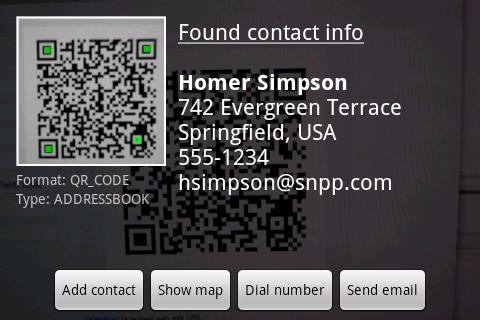
\includegraphics[width=0.6\textwidth]{research/images/zxing_barcode.jpeg}
	
	\caption[ZXing Barcode Scanner]%
    {ZXing Barcode Scanner displaying the result of scanning a QR Code containing contact details.}
	\label{zxing_scanner}
\end{figure}

It is valuable to identify an application at this stage that is capable of performing some form of image analysis on the handset. While the application of the image analysis in this instance is being applied to relatively structured input it is still faced with performance, lighting and optical constraints that are likely to play a factor in this project.

\section{Android OS}
As mentioned earlier in this report, the Google Android platform has gained considerable market penetration in the short few years since its release in 2008. A large number of manufacturers including Samsung, LG, Motorola, HTC and Sony Ericsson have been producing Android based handsets at a vast range of price points and configurations. This variety of available hardware coupled with development for the platform through the Java programming language makes it an appealing platform to develop for.

Google Android is a operating system and software stack, consisting of a modified Linux kernel, a collection of C based libraries offering database, media and 3d graphics to the system and a custom built Java virtual machine called Dalvik. This virtual machine is different to traditional Java VM’s which are traditionally stack based, Dalvik is a register based VM. To execute standard Java classes on the VM \emph{.class} files must be converted to a single Dalvik \emph{.dex}, duplicated data such as strings and constants are removed which helps to conserve space. This conversion process helps to reduce the in memory footprint of an application.

\begin{figure}[h!]
\centering
    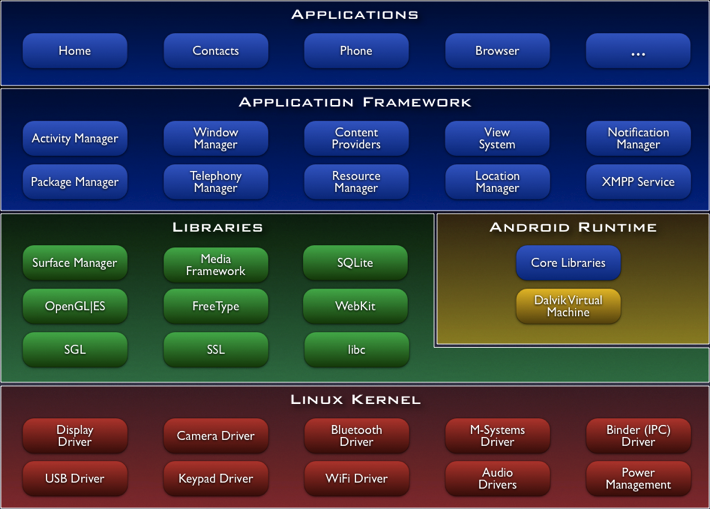
\includegraphics[width=1\textwidth]{research/images/android_arch.png}
	\caption{Android architecture overview}%
	\label{android_arch}
\end{figure}

To begin developing an understanding of the platform a number of tutorials and documents on the developer site \url{developer.android.com} were followed, and they proved to be valuable in getting to grips with the platform. 

\section{Computer Vision}

\subsection{Libraries}

\subsection{Techniques}

\section{JINI and the NDK}

\section{Focus}
